% \documentclass[rmp,aps,floatfix,authordate1-4,preprint]{revtex4}
% \documentclass[prb,aps,floatfix,authordate1-4,preprint]{revtex4}

\documentclass[pre,aps,floatfix,authordate1-4,twocolumn]{revtex4-1}
%\documentclass[pre,aps,floatfix,authordate1-4]{revtex4-1}

%\documentclass[aps,prl,preprint,superscriptaddress]{revtex4}



%\documentclass[aps,prl,preprint,groupedaddress]{revtex4}

\usepackage{rotating} 
\usepackage{times}
\usepackage{graphicx}
\usepackage{setspace}
\usepackage{amsmath}
\usepackage{caption}
\usepackage{subcaption}
\usepackage{epstopdf}
%\usepackage{array}
%\usepackage{arydshln}
%\usepackage[sort&compress]{natbib}
%\bibpunct{(}{)}{,}{n}{}{}
%\renewcommand{\bibnumfmt}[1]{#1.}
\usepackage[obeyFinal]{easy-todo}

\usepackage[normalem]{ulem}

\begin{document}
%\singlespacing

\title{The molecular electrometer and binding of cations to phospholipid bilayers}

\author{Andrea Catte}
%\thanks{The authors are listed in alphaphetical order,The author list is not completed.}
\thanks{University of East Anglia, Norwich, United Kingdom}
\author{Mykhailo Girych}
\thanks{Helsinki Biophysics and Biomembrane Group, Department of Biomedical Engineering and Computational Science, Aalto University, Espoo, Finland}
\author{Matti Javanainen}
\thanks{Tampere University of Technology, Tampere, Finland}
\author{Claire Loison}
%\thanks{Lyon}
\author{Josef Melcr}
\thanks{Institute of Organic Chemistry and Biochemistry, Czech Academy of Sciences, Flemingovo nám. 2, 16610 Prague 6, Czech Republic,
Charles University in Prague, Faculty of Mathematics and Physics, Ke Karlovu 3, 121 16 Prague 2, Czech Republic}
\author{Markus S. Miettinen}
\thanks{Fachbereich Physik, Freie Universit\"at Berlin, Berlin, Germany}
\author{Luca Monticelli}
\thanks{Institut de Biologie et Chimie des Prot{\'e}ines (IBCP), CNRS UMR 5086, Lyon, France}
%\setcounter{page}{1}
\author{Jukka M{\"a}{\"a}tt{\"a}}
\thanks{Aalto University, Espoo, Finland}
\author{Vasily S. Oganesyan}
\thanks{University of East Anglia, Norwich, United Kingdom}
\author{O. H. Samuli Ollila} 
\thanks{{\bf Author to whom correspondence may be addressed. E-mail: samuli.ollila@aalto.fi.},Department of Neuroscience and Biomedical Engineering, Aalto University, Espoo, Finland}
\author{Joona Tynkkynen}
\thanks{Tampere University of Technology, Tampere, Finland}
\author{Sergey Vilov}
%\thanks{Lyon}
%\footnote{Author to whom correspondence may be addressed. E-mail: samuli.ollila@aalto.fi.\\}


\begin{abstract}
Despite the vast amount of experimental and theoretical studies, the binding affinity of cations, especially the 
biologically relevant Na$^+$ and Ca$^{2+}$ ions, into a phosholipid bilayer is not agreed on in the literature. 
Here we show that the ion binding affinity can be directly compared between simulations and experiments by 
using the choline headgroup order parameters according to the 'molecular electrometer' concept.~\cite{seelig87}.

Our results strongly support the pre-2000 view that Na$^+$ and other monovalent ions
(bar Li$^+$) do not specifically bind to phosphatidylcholine lipid bilayers with mM concentrations, 
in contrast to Ca$^{2+}$ and other multivalent ions. Especially the Na$^+$ binding affinity is 
overestimated by several molecular dynamics simulation models, leading to an artificially positively
charged lipid bilayer. Qualitatively correct headgroup order parameter response is observed with
Ca$^{2+}$ binding in all the tested models, however, none of the tested models has sufficient 
quantitative accuracy to interpret the Ca$^{2+}$:lipid stoichiometry or the induced atomistic resolution structural changes.

{\it This work has been, and continues to be, progressed and discussed through the blog \url{nmrlipids.blogspot.fi},
through which everyone is invited to join the discussion and make contributions. The manuscript will be
eventually submitted to an appropriate scientific journal. Everyone who has contributed to the work through the
blog will be offered coauthorship. For more details see \url{nmrlipids.blogspot.fi}.}
\end{abstract}


\maketitle


~\vspace{0.3cm}\\
{\it \bf} 

\section{Introduction}

Due to its high physiological importance --- nerve cell signalling being the prime example ---
interaction of cations with phospholipid membranes
has been widely studied via theory, simulations, and experiments.
It is generally agreed that the relative binding affinities of different ions 
follow the Hofmeister series~\cite{eisenberg79,cevc90,tocanne90,binder02,celma07,leontidis09,vacha09a,klasczyk10,harb13}, 
however,
consensus on the quantitative binding affinities is currently lacking.
Two extensive reviews covering the field until 1990~\cite{cevc90,tocanne90}
demonstrate that until that time it was generally considered that
while  multivalent cations interact significantly with phospholipid bilayers,
for monovalent cations (with the exception of Li$^+$) the interactions are weak.
This conclusion has since been further supported by contemporary
studies showing that bilayer properties remain unaltered upon addition of millimolar concentrations of monovalent 
salt~\cite{binder02,pabst07,filippov09}. 
However, since 2000, another view, questioning the weakness of interactions between phospholipids and monovalent cations
and suggesting a much stronger binding especially for Na$^{+}$, has emerged
%in several experimental and molecular dynamics simulation studies~
\cite{bockmann03,bockmann04,vacha09a,manyes05,manyes06,fukuma07,leontidis09,ferber11,morata12,klasczyk10,harb13}.

The pre-2000 view is supported by the experimental findings that
(in contrast to significant effects by the presence of CaCl$_2$ or other multivalent ions)
millimolar concentrations of NaCl have a negligible effect on
phospholipid infrared spectra~\cite{binder02},
area per molecule~\cite{pabst07},
dipole potential~\cite{clarke99},
lipid lateral diffusion~\cite{filippov09},
and choline head group order parameters~\cite{akutsu81}.
% [reference to be added?]
In addition, water sorption isotherms for a POPC/NaCl system and NaCl in pure water are very similar
--- indicating only weak interaction between ions and lipids~\cite{binder02}. %Further, only minor changes in POPC infrared spectra are observed in the presence of NaCl, while changes are significant in the presence of Ca$^{2+}$ and other multivalent ions,  also confirming that interaction between Na$^+$ and lipids are weak~\cite{binder02}.

The post-2000 view, which in contrast suggests strong Na$^{+}$ binding, rests on experimental and simulational findings.
The rotational and translational dynamics of fluorescent probes in lipid bilayers decrease with mM NaCl concentrations~\cite{bockmann03,vacha09a,harb13}, and bilayer hardness and area per lipid measured with Atomistic Force Microscopy (AFM) change~\cite{manyes05,manyes06,fukuma07,ferber11,morata12}.
In addition, atomistic molecular dynamics (MD) simulations
commonly predict binding of Na${^+}$ ions 
to phoshatidylcholine lipid bilayers, although the strength of binding depends on the specific model used~\cite{bockmann03,bockmann04,sachs04,berkowitz06,cordomi08,cordomi09,valley11,berkowitz12}. 
%Generally the CHARMM based force fields predict less Na$^+$ binding and changes in bilayer
%properties than the GROMOS based force fields~\cite{sachs04,valley11}.
Upon Na$^+$ binding, some simulation studies reported a reduction in lipid lateral diffusion, 
{\it in agreement with the fluorescent probe measurements~\cite{bockmann03,vacha09a,harb13}}.
%but in contrast with NMR experiments~\cite{filippov09}. 
Other simulations showed a reduction in area per lipid in the presence of NaCl, 
{\it in agreement with AFM experiments~\cite{manyes05,manyes06,fukuma07,ferber11,morata12};
however, the reduction in area was observed at excessively low Na$^+$ concentrations, 
compared to observations from scattering experiments~\cite{pabst07}}.
Predictions of electrophoretic mobility in the presence of NaCl yielded positive values, higher than in experiments; 
however, this could be explained by the behaviour of Cl$^-$ ions~\cite{berkowitz06,knecht13}.

Some observables have been interpreted to favor both the pre- as well as the post-2000 views.
For example, while the reduced lateral diffusion of fluorescent probes was interpreted to support the post-2000 view,
reduction of lipid diffusion was not observed in noninvasive NMR experiments,
suggesting that fluorescence results arise from Na$^{+}$ interactions with probes rather than with lipids~\cite{filippov09}.
And  %have been interpreted to support both sides:
as the effect of monovalent ions (bar Li$^+$)  on the phase transition temperature is 
(compared to the effect of multivalent ions) small, it was initially interpreted %by Cevc
as an indication that only multivalent ions and Li$^+$ specifically bind to phosholipid bilayers~\cite{cevc90}; 
however, more recently such small effect in calorimetric measurements was interpreted to indicate that 
also Na$^+$ binds~\cite{bockmann03,klasczyk10}.
Finally, in electrophoresis measurements on phosphatidylcholine vesicles, 
positive zeta potentials can be generally reached only with multivalent ions or Li$^+$,
whereas NaCl increases the (initially negative) zeta potential to only about zero~\cite{eisenberg79,tatulian87,manyes05,manyes06,klasczyk10}. 
This lack of significant positive electrophoretic mobility in the presence of NaCl suggested weak binding of Na$^+$; 
however, the same data has also been explained by an effect of the Cl$^-$ ions~\cite{berkowitz06,knecht13}.

In the present work we set out to solve the apparent contradictions
between the pre-2000 and post-2000 views
by directly comparing the headgroup hydrocarbon segment
$\alpha$ and $\beta$ (see Fig. \ref{POPCstructure}) order parameters between simulations
and experiments as a function of cation concentration. 
According to the 'molecular electrometer' concept, changes in order parameters of the $\alpha$ and $\beta$ carbons 
in the phospholipid head group can be used to measure the ion affinity to the 
phophatidylcholine (PC) lipid bilayer~\cite{akutsu81,altenbach84,seelig87,scherer89}.
Order parameters can be accurately measured in experiments and straightforwardly compared to 
simulations \cite{ollila16}, therefore the molecular electrometer allows the 
comparison of binding affinity between simulations and experiments. 
We show that the response of order parameters to penetrating cations 
is qualitatively correct in simulations, but the affinity of PC bilayers for Na$^{+}$ ions 
is significantly overestimated in several MD simulation models. 
Moreover, we show that the accuracy of tested models does not allow for
an interpretation of lipid--Ca$^{2+}$ interactions with atomistic resolution.



\begin{figure}[]
  \centering
  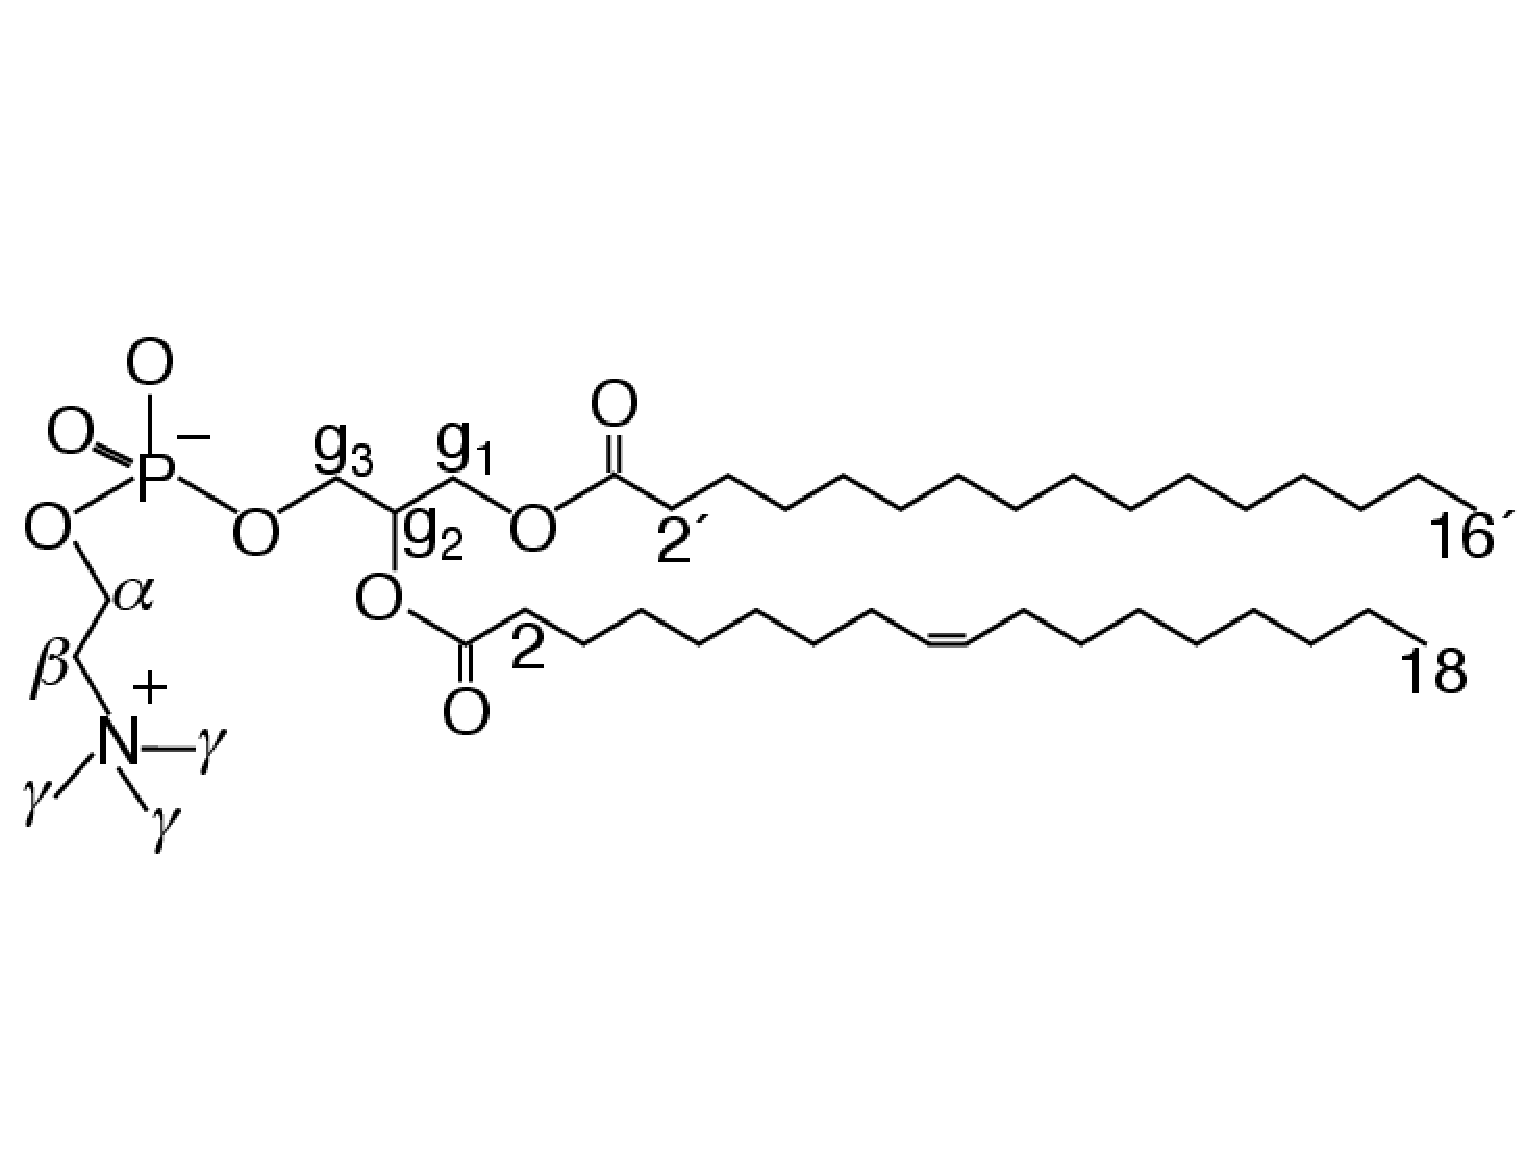
\includegraphics[width=8.6cm]{../Fig/POPCstructure.eps}

  \caption{\label{POPCstructure}
    Chemical structure of 1-palmitoyl-2-oleoylphosphatidylcholine (POPC).}
  
\end{figure}





\section{Results and Discussion}

\subsection{Molecular electrometer concept in experiments}\label{conceptinexperiments}
According to the molecular electrometer concept the binding of charged objects on 
PC bilayer interface induce systematic changes in choline $\beta$ and $\alpha$
segment order parameters. Thus, the changes of these order parameters can be used
to determine binding affinities of the charged objects. The concept is originally
based on experimentally observed changes in choline order parameters with bound 
cations~\cite{akutsu81,altenbach84}, see Fig. \ref{ordPions} for data as a function
of ion concentration in solution. 
\begin{figure*}[]
  \centering
  \includegraphics[width=15cm]{../Fig/OrderParameterIONSchanges.eps}
  \caption{\label{ordPions}
    The order parameter changes for $\beta$ and $\alpha$ segments as a function of NaCl (left column) 
    and CaCl$_2$ (right column) concentration, from simulations and experiments~\cite{akutsu81} 
    (POPC with CaCl$_2$ from \cite{altenbach84}). The signs of the experimental order parameters, taken from
    experiments without ions~\cite{hong95a,hong95b,gross97}, can be assumed to be unchanged 
    with concentrations represented here~\cite{altenbach84,ollila16}. 
    It should be noted that none of the models used here reproduces the order parameters
    within experimental error for pure PC bilayer without ions, indicating structural inaccuracies with varying severity in all
    models \cite{botan15}. %this is important to say, otherwise someone might get wrong impression from this fig.
    Note that the relatively large decrease in CHARMM36 with 450~mM CaCl$_2$ arise from more equilibrated binding 
    affinity due to long simulation times, see supplementary information.
  }
\end{figure*}

Further quantification with various positively 
and negatively charged molecules showed that choline order parameters vary linearly 
with small amount of bound charge per lipid~\cite{altenbach84,altenbach85,seelig87,macdonald87,scherer89,roux90,beschiasvili91,marassi92,rydall92}.
%Since the quadrupolar splitting is $\Delta\nu_i^{\rm{Q}}=-\frac{3}{4} \chi S_{\rm{CD}}$
%and $S_{\rm{CD}} \approx S_{\rm{CH}}$~\cite{ollila16} 
The relation between bound charge per lipid $X^\pm$ and choline order parameters can be then written as~\cite{ferreira16}
\begin{equation}\label{electrometer_eq}
S_{\rm{CH}}^{i}(X^\pm)=S_{\rm{CH}}^{i}(0) + \frac{4}{3}\chi^{-1}m_i X^\pm,
\end{equation}
where the quadrupole coupling constant $\chi$ is approximately equal to 167 kHz,
$S_{\rm{CH}}^{i}(0)$ is order parameter without bound charges, $m_i$
is constant depending on the valency and position of bound charge, and $i$
refers to either $\alpha$ or $\beta$. The order parameter change respect to a 
bilayer without bound charges then becomes
\begin{equation}\label{OPchangeEQ}
\Delta S_{\rm{CH}}^{i}= S_{\rm{CH}}^{i}(X^\pm)-S_{\rm{CH}}^{i}(0) =\frac{4}{3}\chi^{-1}m_i X^\pm.
\end{equation}
Combination of atomic absorption spectra and $^2$H NMR experiments gave $m_\alpha=-20.5$ 
and $m_\beta=-10.0$ for Ca$^{2+}$ binding in POPC bilayer in the presense of 100mM NaCl~\cite{altenbach84}.

The quantification of $\beta$ and $\alpha$ segment order parameter changes 
with different cations
have revealed that $\Delta S_{\rm{CH}}^{\beta}/\Delta S_{\rm{CH}}^{\alpha} \approx0.5$ for wide range
of different cations (aqueous cations, cationic peptides, cationic anesthetics)~\cite{beschiasvili91,rydall92}.
More specifically, the experimental data shown in Fig.~\ref{AvsB} led to the 
relation $\Delta S_{\rm{CH}}^{\beta}=0.43\Delta S_{\rm{CH}}^{\alpha}$ for DPPC bilayer
with various CaCl$_2$ concentrations~\cite{akutsu81}.
\begin{figure}[]
  \centering
  \includegraphics[width=8cm]{../Fig/OrderParameterAvsB.eps}
  \caption{\label{AvsB}
    Relation between $\Delta S_{\rm{CH}}^{\beta}$ and $\Delta S_{\rm{CH}}^{\alpha}$ from experiments~\cite{akutsu81} and
    different simulation models. Solid line is $\Delta S_{\rm{CH}}^{\beta}=0.43\Delta S_{\rm{CH}}^{\alpha}$ determined for DPPC bilayer
    from $^2$H NMR experiment with various CaCl$_2$ concentrations~\cite{akutsu81}.
  }
\end{figure}
%With these values the Eq.~\ref{electrometer_eq} gives
%\begin{equation}\label{alphaCH}
%\Delta S_{\rm CH}^\alpha=-0.16 X^{\rm Ca^{2+}}
%\end{equation}
%and
%\begin{equation}\label{betaCH}
%\Delta S_{\rm CH}^\beta=-0.08 X^{\rm Ca^{2+}},
%\end{equation}
%where $X^{\rm Ca^{2+}}$ is the amount of bound Ca$^{2+}$ per lipid.
%Order parameter changes a function of bound charges from Eqs. \ref{alphaCH} and
%\ref{betaCH} are shown in Fig.~\ref{electrometer}. 

In original experiments the absolute values of order parameters 
increased for $\beta$ and decreased for $\alpha$ segment with bound positive charge
and {\it vice versa} for negative charge~\cite{akutsu81,altenbach84,altenbach85,seelig87,scherer89,rydall92}. 
However, it is now known that 
$\beta$ carbon order parameter is negative while $\alpha$ carbon order parameter is 
positive~\cite{hong95a,hong95b,gross97}. Thus, we can conclude 
that $\beta$ and $\alpha$ segment order parameters decrease with bound positive charges 
and increase with bound negative charge. Consequently, values of $m_i$ are negative for
bound positive charges and {\it vice versa}. This can be rationalized by electrostatically 
induced changes in choline P-N dipole tilt \cite{seelig87,scherer89,seelig90} which is also
seen in simulations~\cite{cordomi08,cordomi09,zhao12}. This is in line with order parameter decrease 
related to the P-N vector tilting more parallel to membrane plane seen with decreased hydration levels~\cite{botan15}. 

%, and positive to the 
%sign to the order parameter of the 
%carbon
%thus both order parameter values are actually decreasing %(becoming more negative) 
%as the concentration of cations increases~\cite{ollila15}. 
%Combining extensive quantitifaction of electrometer concept with
%were measured \cite{akutsu81,altenbach84,seelig87,scherer89}
%order current knowledge on order parameter signs~\cite{hong95a,hong95b,gross97}, 

The headgroup order parameter changes as a function of ion concentration in
solution from H$^2$ NMR experiments are shown in Fig.~\ref{ordPions} for DPPC and POPC bilayers~\cite{akutsu81,altenbach84}.
%with correct signs~\cite{hong95a,hong95b,gross97}, 
%as a function NaCl and CaCl$_2$ concentration. 
In contrast to the response as a function of bound charge in 
Eq. \ref{electrometer_eq}, the changes in Fig. \ref{ordPions}
are not linear. This can be explained by electrostatic repulsion between
already bound Calcium ions and ions in solution \cite{altenbach84}.
Experimental data in Fig. \ref{ordPions} shows only minor changes in order
parameter as a function of NaCl is solution, 
while the effect of CaCl$_2$ is an order of magnitude larger. 
Thus, according to the molecular electrometer concept, 
monovalent Na$^+$ ions have negligible affinity for PC lipid bilayers at concentrations up to 1 M,
while binding of Ca$^{2+}$ ions at the same concentration is significant~\cite{akutsu81,altenbach84}. 
This conclusion is in agreement with several other experimental 
studies~\cite{cevc90,tocanne90,binder02,pabst07,filippov09}.

\subsection{Molecular electrometer concept in MD simulations}\label{electrometerinsimulations}

Figure~\ref{ordPions} also reports order parameter changes calculated from MD simulations
of DPPC and POPC lipid bilayers as a function of NaCl or CaCl$_2$ concentrations in solution. 
Details of the simulated systems are reported in Table~\ref{IONsystems} and in Supplementary Information. 
It should be noted that none of the models used here 
reproduced the order parameters for pure PC bilayer without ions 
within experimental uncertainty in our previous study (Figure 2 in Ref. \cite{botan15}), 
indicating structural inaccuracies with varying severity for all models \cite{botan15}.
%\todo{MONTICELLI: hmm, I see a little problem here: the absolute values for the order parameters are not reported here,
% so how can we notice that they don't match the experiment? 
% Is it worth having another figure? If not, then I will rephrase this bit above, I don't think it's very clear. \\
%OLLILA: This is now modified to explicitly point the fig. 2 in NMRlipids I paper.
%https://github.com/NMRLipids/lipid\_ionINTERACTION/issues/3 }
On the other hand, the experimentally observed headgroup order parameter increase with dehydration
was qualitatively reproduced by all the tested models \cite{botan15}. 
Accordingly, the presense of cations in simulations leads to the decrease 
of choline order parameters in Fig. \ref{ordPions}, which is in qualitative
agreement with experiments. However, the changes are overestimated in most
simulation results in Fig \ref{ordPions}. 

According to the electrometer concept the order parameter changes are proportional to
the amount of bound cations in bilayer, see Eq. \ref{OPchangeEQ}.
The order parameter changes as a function of bound charge from simulations are
shown in Fig. \ref{electrometer}. Roughly linear correlation between bound charge
and order parameter change is found in all simulation models, which is in line with
experiments \cite{altenbach84}. However, there are some differences in the 
proportionality constans (i.e. slopes in Fig. \ref{electrometer}) between different
models; especially MacRog and Orange models give relatively steep slopes and CHARMM
gives gentle slope for $\alpha$ carbon. The quantitative comparison to experimental
slopes ( $m_\alpha=-20.5$ and $m_\beta=-10.0$ for Ca$^{2+}$ binding in DPPC bilayer in
the presense of 100mM NaCl in Eq. \ref{electrometer_eq}~\cite{altenbach84}) is not straightforward 
since the simulation results depend on the definition used for bound ions. 
%Thus the more detailed analysis is left for further studies.
\begin{figure}[]
  \centering
  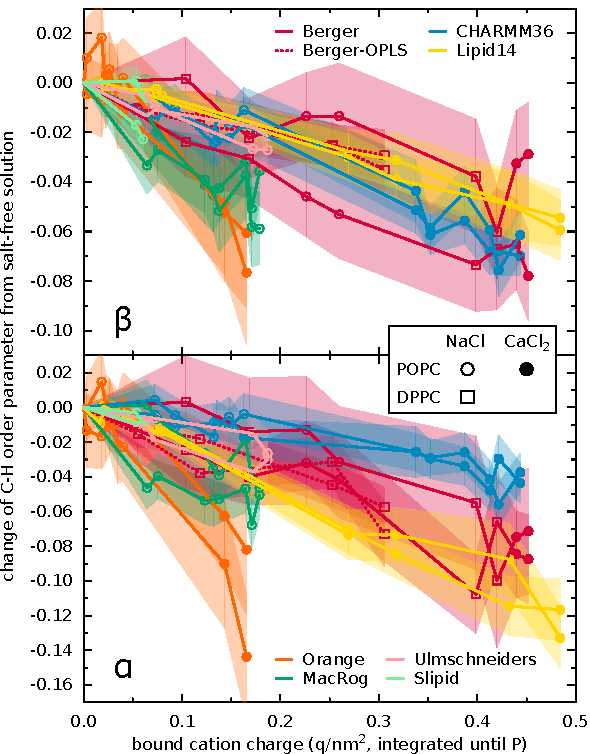
\includegraphics[width=8.6cm]{../scratch/boundIons/dOP_vs_boundCationCharge_P.pdf}
  \caption{\label{electrometer}
    Order parameters changes $\Delta S_{\rm{CH}}^{\beta}$ and $\Delta S_{\rm{CH}}^{\alpha}$ as a function of bound
    cations from different simulation models.
   }
\todo{Results from long CHARMM and Slipids simulations to be added. Description of the calculation of bound charges to be described, probably in supplementary.}
\end{figure}

The comparison of order parameter changes as a function of bound charge is more straightforward for
systems with charged amphihiles, which are fully associated in bilayer. In this case the amount of bound charge
is explicitly known in both, simulations and experiment. Such comparison is done 
between previously published simulation data \cite{miettinen09} and experiments \cite{scherer89,franzin98}
in Supplementary Information. The overestimation of order parameter response to bound cations (i.e. slopes $m_\beta$ and $m_\alpha$)
could not be ruled out in the Berger based model. In principle, this might explain the overestimated order parameter 
response to CaCl$_2$ with Berger model, but not overestimated response to NaCl (see discussion in Supplementary Information).
The more detailed comparison with different models is left for further studies.



%The order parameter changes as a function of cationic amphiphiles
%in bilayer is compared between previously published Berger based simulations (DMPC with cationic dimyristoyltrimethylammoniumpropane
%(DMTAP))~\cite{miettinen09} and experiments~\cite{scherer89,franzin98} in Supplementary Information. The response in simulations is 
%similar as the average of various cationic amphiphiles measured by Scherer et al.~\cite{scherer89} but larger 
%than response of POPC bilayer measured with 1,2-dioleoyloxy-3-(trimethylammonio)propane (DOTAP).


The relation between $\Delta S_{\rm{CH}}^{\beta}$ and $\Delta S_{\rm{CH}}^{\alpha}$ from different simulation models
is compared to experiments in Fig.~\ref{AvsB}. Almost all the tested models give larger $\Delta S_{\rm{CH}}^{\beta}/\Delta S_{\rm{CH}}^{\alpha}$ ratio
than in experiments~\cite{akutsu81}; only Lipid14 give values in agreement with experimental ratio.
Thus, in all the other tested simulation models $\alpha$ order parameter decrease is underestimated in
respect to $\beta$ order parameter decrease with bound cations.

Figure \ref{electrometer} shows that order parameter decrease clearly correlates with the
amount of bound cations also in simulations. This is also evident from Fig.~\ref{NAdensities}
showing Na$^+$ density profiles from the different simulation models. 
In the figure, simulation models are ordered according to the order parameter changes 
(reported Fig.~\ref{ordPions}), from the smallest to the largest.
The Na$^+$ density peaks are larger for models with larger changes in order parameters,
in line with observed correlation between cation binding and order parameter decrease in
Fig. \ref{electrometer}.

In conclusion, the clear correlation between bound cations and order parameter decrease 
is observed in all the tested simulation models. However, quantitative responses of $\alpha$ and $\beta$
on bound cations do not generally agree with experiments because the $\Delta S_{\rm{CH}}^{\beta}/\Delta S_{\rm{CH}}^{\alpha}$ ratio  
agrees with experiments only in Lipid14 model (Fig.~\ref{AvsB}). Thus, the observed 
overestimations of order parameter changes with cation concentrations may, in principle, arise
from overbinding of ions or from too sensitive lipid headgroup response on bound cation 
(see also discussion in Supplementary Material). Consequently, the electrometer concept can be 
used to quantitatively compare the cation binding affinity between experiments and simulations, 
but careful analysis is required with current lipid models. Such analysis is performed in the next section.


\begin{table*}[htb]
\centering
\caption{List of simulations performed in this work. The ion concentrations are calculated as 
   [ion]=(N$_{\rm ion} \times$[water])/N$_{\rm w}$, where [water]=55.5M. 
   These correspond the concentrations reported in the experiments by Akutsu et al.~\cite{akutsu81}.
   The lipid force fields are named as in our previous work~\cite{botan15}.}\label{IONsystems}
\begin{tabular}{c c c c c c c c c c c c}
  %\hline
  Force field (lipid, ion)& lipid & [Ion] mM & \footnote{The number of lipid molecules}N$_{\rm l}$   &  \footnote{The number of water molecules}N$_{\rm w}$   & \footnote{The number of Na$^+$ molecules}N$_{\rm Na}$  & \footnote{The number of Ca$^{2+}$ molecules}N$_{\rm Ca}$   &  \footnote{The number of Cl molecules}N$_{\rm Cl}$ & \footnote{Simulation temperature}T (K)  & \footnote{The total simulation time}t$_{{\rm sim}}$(ns) & \footnote{Time frames used in the analysis}t$_{{\rm anal}}$ (ns) & Files\\
  \hline
  Berger-POPC-07\cite{ollila07a}   &   POPC & 0          & 128 & 7290 & 0  & 0  & 0 & 298  & 270 & 240 & \cite{bergerFILESpopc}  \\
  Berger-POPC-07\cite{ollila07a}, ffgmx\cite{straatsma88}  &   POPC & 340 (NaCl) & 128 & 7202 & 44  & 0  & 44 &298  & 110 & 50 & \cite{bergerPOPC340mMNaClfiles} \\
  %\hdashline
  Berger-POPC-07\cite{ollila07a}, ffgmx\cite{straatsma88}  &   POPC & 340 (CaCl$_2$) & 128 & 7157 & 0 & 44  & 88 &298 & 108 & 58 &\cite{bergerPOPC340mMCaClfiles}  \\
  \hline
  Berger-DPPC-97\cite{marrink98}   &   DPPC & 0 & 72 & 2880 & 0  & 0  & 0 &323  & 60 & 50 &\cite{bergerDPPCfiles} \\
  Berger-DPPC-97\cite{marrink98}, ffgmx\cite{straatsma88}   &   DPPC & 150 (NaCl) & 72 & 2880 & 8  & 0  & 8 &323  & 120 & 60 &\cite{bergerDPPC150mMfiles} \\
  Berger-DPPC-97\cite{marrink98}, ffgmx\cite{straatsma88}   &   DPPC & 1000 (NaCl) & 72 & 2778 & 51  & 0  & 51 &323  & 120 & 60 &\cite{bergerDPPC1000mMfiles} \\
  \hline
  BergerOPLS-DPPC-06\cite{tieleman06} &   DPPC & 0 & 72 & 2880 & 0  & 0  & 0 &323  & 120 & 60 &\cite{bergerOPLSDPPCfiles} \\
  BergerOPLS-DPPC-06\cite{tieleman06}, OPLS\cite{aqvist90} &   DPPC & 150 (NaCl) & 72 & 2880 & 8  & 0  & 8 &323  & 120 & 60 &\cite{bergerOPLSDPPCfiles150mMnacl} \\
  BergerOPLS-DPPC-06\cite{tieleman06}, OPLS\cite{aqvist90} &   DPPC & 1000 (NaCl) & 72 & 2778 & 51  & 0  & 51 &323  & 120 & 60 &\cite{bergerOPLSDPPCfiles1000mMnacl} \\
  \hline
  CHARMM36\cite{klauda10}   & POPC & 0           & 72 & 2242 & 0  & 0 & 0 & 303  & 30 & 20 & \cite{charmm36filesSHORT} \\
  CHARMM36\cite{klauda10}, CHARMM36\cite{venable13} & POPC & 350 (NaCl)  & 72 & 2085 & 13  & 0 & 13 & 303  & 80 & 60 & \cite{charmmPOPC350mMNaClfiles} \\
  CHARMM36\cite{klauda10}, CHARMM36\cite{venable13} & POPC & 690 (NaCl)  & 72 & 2085 & 26  & 0 & 26 & 303  & 73 & 60 & \cite{charmmPOPC690mMNaClfiles}   \\
  CHARMM36\cite{klauda10}, CHARMM36\cite{venable13}  & POPC & 950 (NaCl)  & 72 & 2168 & 37  & 0 & 37 & 303  & 80 & 60 &\cite{charmmPOPC950mMNaClfiles}  \\
  %CHARMM36\cite{klauda10}, ionFF~\cite{??}\todoi{Appropriate reference for the ion model?}  & POPC & 1380 (NaCl)  & 72 & 2085 & 52  & 0 & 52 & 303  & 80 & 60 &?\todoi{Samuli put to Zenodo} \\
  %CHARMM36\cite{klauda10}, ionFF~\cite{??}\todoi{Appropriate reference for the ion model?}   & POPC & 2080  (NaCl)  & 72 & 2085 & 78  & 0 & 78 & 303  & 73 & 60 &?\todoi{Samuli put to Zenodo} \\
  CHARMM36\cite{klauda10}, CHARMM36 & POPC &  350 (CaCl$_2$)  & 128 & 6400 & 0& 35 & 70 & 303  & 200  & 100 & \cite{charmmPOPC350mMCaClfiles}  \\
  CHARMM36\cite{klauda10}, CHARMM36 & POPC &  450 (CaCl$_2$)  & 200 & 9000 & 0& 73 & 146 & 310  & 2000  & 100 & \cite{charmmPOPC450mMCaClfiles}  \\
  CHARMM36\cite{klauda10}, CHARMM36 & POPC &  670 (CaCl$_2$)  & 128 & 6400 & 0& 67 & 134 & 303  & 200  & 120 & \cite{charmmPOPC670mMCaClfiles}  \\  
  CHARMM36\cite{klauda10}, CHARMM36 & POPC &  1000 (CaCl$_2$) & 128 & 6400 & 0& 100 & 200 & 303 & 200  & 100 & \cite{charmmPOPC1000mMCaClfiles}  \\
  \hline
  CHARMM36\cite{klauda10}, Yoo\cite{yoo16}  & DPPC & 430 (CaCl$_2$)  & 128 & 7760 & 60  & 0 & 120 & 323  & 200 & 170 &todo  \\
  CHARMM36\cite{klauda10}, Yoo\cite{yoo16}  & DPPC & 886 (CaCl$_2$)  & 128 & 7520 & 120  & 0 & 240 & 323  & 200 & 170 &todo  \\
  \hline
  MacRog\cite{maciejewski14}  & POPC & 0 & 288 & 14400 & 0 & 0 & 0 & 310 & 90&40  &~\cite{macrogdehydFILES}  \\
  MacRog\cite{maciejewski14}, OPLS\cite{aqvist90}  & POPC & 100 (NaCl) & 288 & 14554 & 27 & 0 & 27 & 310 & 90&50  & \cite{macrogIONfiles} \\
  MacRog\cite{maciejewski14}, OPLS\cite{aqvist90}  & POPC &  210 (NaCl) & 288 & 14500 & 54 & 0 & 54 & 310 & 90&50  &\cite{macrogIONfiles}  \\
  MacRog\cite{maciejewski14}, OPLS\cite{aqvist90}  & POPC &   310 (NaCl) & 288 & 14446 & 81 & 0 & 81 & 310 & 90&50  & \cite{macrogIONfiles} \\
  MacRog\cite{maciejewski14}, OPLS\cite{aqvist90}  & POPC &   420 (NaCl) & 288 & 14392 & 108 & 0 & 108 & 310 & 90& 50  & \cite{macrogIONfiles}  \\
  \hline
  Orange, OPLS\cite{aqvist90}  &   POPC & 0 & 72 & 2880 & 0 & 0  & 0 & 298 & 60 & 50 & \cite{orangePOPCfiles}  \\
  Orange, OPLS\cite{aqvist90} &   POPC & 140 (NaCl) & 72 & 2866 & 7 & 0  & 7 & 298 & 120 & 60 &\cite{orangePOPC140mMNaClfiles}  \\
  Orange, OPLS\cite{aqvist90}  &   POPC & 510 (NaCl) & 72 & 2802 & 26 & 0  & 26 & 298 & 120 & 100 &\cite{orangePOPC510mMNaClfiles}   \\
  Orange, OPLS\cite{aqvist90}  &   POPC & 1000 (NaCl) & 72 & 2780 & 50 & 0  & 50 & 298 & 120 & 80 & \cite{orangePOPC1000mMNaClfiles} \\
  %\hdashline
  Orange, OPLS &   POPC & 510 (CaCl$_2$)  & 72 & 2802 & 0 & 26  & 52 & 298 & 120 & 60 & \cite{orangePOPC510mMCaClfiles}  \\
  \hline
  Slipid\cite{jambeck12}   &   DPPC & 0 & 128 &3840 & 0 & 0  & 0 & 323 & 150 & 100 &~\cite{slipidsFILES}  \\
  Slipid\cite{jambeck12}, AMBER\cite{beglov94,roux96} &   DPPC & 150 (NaCl) & 600 & 18000 & 49 & 0  & 49 & 323 & 100 & 40 &-  \\
  Slipid\cite{jambeck12}, AMBER\cite{beglov94,roux96} &   DPPC & 350 (NaCl) & \todo{J. Melcr, please fill}? & ? & ? & 0  & ? & ? & ? & ? & ?  \\
  Slipid\cite{jambeck12}, AMBER\cite{beglov94,roux96} &   DPPC & 700 (NaCl) & ? & ? & ? & 0  & ? & ? & ? & ? & ?  \\
  Slipid\cite{jambeck12}, AMBER\cite{beglov94,roux96} &   DPPC & 1000 (NaCl) & ? & ? & ? & 0  & ? & ? & ? & ? & ?  \\
  \hline
  Slipid\cite{jambeck12b}   &   POPC & 0 & 128 & 5120 & 0 & 0  & 0 & 303 & 200 & 150 &~\cite{slipidsFILESpopc}  \\
  Slipid\cite{jambeck12b}, AMBER\cite{smith94}  &  POPC & 130 (NaCl) & 200 & 9000 & 21 & 0  & 21 & 310 & 105 & 100 &~\cite{slipidsFILESpopc130mMnaclSD}  \\
  Slipid\cite{jambeck12b}, AMBER\cite{aqvist90}  &  POPC & 450 (CaCl) & 200 & 9000  & 0 & 73  & 146 & 310 & 2000 & 100 &~\cite{slipidsFILESpopc450mMcacl}  \\
  \hline
  Lipid14~\cite{dickson14}, AMBER\cite{aqvist90}  &   POPC & 0          & 128 & 5120 & 0 & 0  & 0 & 298 & 205 & 200 &~\cite{lipid14POPC0mMNaClfiles}  \\
  Lipid14~\cite{dickson14}, AMBER\cite{aqvist90}   &   POPC & 150 (NaCl) & 128 & 5120 & 12 & 0 & 12 & 298 & 205 & 200 &~\cite{lipid14POPC150mMNaClfiles}  \\
  Lipid14~\cite{dickson14}, AMBER\cite{aqvist90}   &   POPC & 1000 (NaCl) & 128 & 5120 & 77 & 0 & 77 & 298 & 205 & 200 &~\cite{lipid14POPC1000mMNaClfiles}  \\
  Lipid14~\cite{dickson14}, AMBER\cite{aqvist90}   &   POPC & 350 (CaCl$_2$) & 128 & 6400 & 0 & 35 & 70 & 298 & 200 & 100 &~\cite{lipid14POPC350mMCaClfiles}  \\
  Lipid14~\cite{dickson14}, AMBER\cite{aqvist90}   &   POPC & 1000 (CaCl$_2$) & 128 & 6400 & 0 & 100 & 200 & 298 & 200 & 100 &~\cite{lipid14POPC1000mMCaClfiles}  \\
  \hline
  Ulmschneiders~\cite{Ulmschneider09}, OPLS\cite{aqvist90}       &   POPC & 0          & 128 & 5120 & 0 & 0  & 0 & 298.15 & 205 & 200 &~\cite{ulmschneiderPOPC0mMNaClfiles}  \\
  Ulmschneiders~\cite{Ulmschneider09}, OPLS\cite{aqvist90}       &   POPC & 150 (NaCl) & 128 & 5120 & 12 & 0  & 12 & 298.15 & 205 & 200 &~\cite{ulmschneiderPOPC150mMNaClfiles}  \\
  Ulmschneiders~\cite{Ulmschneider09}, OPLS\cite{aqvist90}       &   POPC & 1000 (NaCl) & 128 & 5120 & 77 & 0  & 77 & 298.15 & 205 & 200 &~\cite{ulmschneiderPOPC1000mMNaClfiles}  \\
\end{tabular}
\end{table*} 




\begin{figure}[]
  \centering
  \includegraphics[width=8cm]{../Fig/NAdensities.eps}
  \caption{\label{NAdensities}
    Atom number density profiles along the membrane normal for lipids, Na$^+$, and Cl$^-$ ions 
    from simulations with different force fields and different NaCl concentrations. 
    The force fields are ordered according to the order parameter changes 
    reported Fig.~\ref{ordPions}, from the smallest (top panel) to the larges (bottom panel).
    The lipid densities are scaled by 100 (united atom) or 200 (all atom model) to improve readability. 
    Figure discussed in https://github.com/NMRLipids/lipid\_ionINTERACTION/issues/4.}
    % are you sure you want to keep this comment (last line) in the submitted paper? 
    % I would prefer to leave it out, as the paper should be self-contained as much as possible.
    % THAT LINE WILL BE REMOVED BEFORE SUBMISSION BUT KEPT AS LONG AS THE DISCUSSION IS GOING ON.
\end{figure}



\subsection{Cation binding in different simulation models}
The order parameter changes and density distributions in Figs.~\ref{ordPions} and \ref{NAdensities} 
with added NaCl show significantly different Na$^+$ binding affinities for different simulation models.
The best agreement with experiments (i.e., lowest order parameter changes) is observed for the Orange,
CHARMM36 and Lipid14 models (see Figs.~\ref{ordPions}). These also predict the lowest Na$^+$ densities 
in the proximity of the membrane (see Fig.~\ref{NAdensities}). On the other hand, the choline order parameter 
changes with NaCl are clearly overestimated in all the other tested models (see Fig.~\ref{ordPions}) which also
show stronger Na$^+$ binding affinity (see Fig.~\ref{NAdensities}). 
%Since binding affinities clearly correlate with order parameter changes between different models and the 
%headgroup sensitivity tested in Supplementary Information cannot explain overestimated order parameter change with NaCl,
Thus we conclude that the sodium binding affinity is overestimated in all the other models than Orange, CHARMM36 and Lipid14. 

The order parameter changes with NaCl in the best three models are small (less than 0.02). Thus, with the achieved accuracy we cannot conclude 
which of these three models has the most realistic Na$^+$ binding affinity, especially with physiological NaCl concentrations ($\sim$ 150mM) 
which is relevant for most applications. 
%This can be explained by unrealistically strong Na$^+$ binding affinity to the bilayer in these models (see Fig.~\ref{NAdensities}). 
The overestimated binding on the other models raise questions on the quality of the predictions from these models when NaCl is present.
%reported in a number of simulation papers... [complete with examples] 
\todo{It has been suggested that we should add references here. The problem is that there are a lot of them and
it is difficult to choose which ones to pick. Any opinions?}
Especially interactions between charged molecules and lipid bilayer might be significantly
affected by the strong Na$^+$ binding which makes bilayer effectively positively charged.

%While the predicted changes in order parameters for these three models are very similar,
%the ion density profiles show differences in Na$^+$ affinity, Orange having lowest affinity and CHARMM36 the highest. 
%With the achieved accuracy for the order parameters we are not able to conclude 
% is this correct? the numbers at low NaCl concentrations are difficult to read.
% SAMULI: Almost all the points are within the error bars. One could say that CHARMM is maybe 
% changing more than others, then there is this weird one point in ORANGE, etc. 
% I think it is beyond the scope to start distinguish these three models since
% in that case we should run more to get smaller error bars and do many other things
% more carefully as well

%\todo{I DID NOT GET THIS: \\
%On one hand, it is clear that models in better agreement with experimental  data on order parameters
%show low Na$^+$ binding affinity, as reported in a number of experiments. 
%On the other hand, differences in ion binding affinities raise questions on the quantitative application 
%of the molecular electrometer in molecular simulations.\\
%IF YOU ARE REFERRING TO THE DIFFERENCES BETWEEN THE BEST THREE MODELS, I THINK THE
%PROBLEM TO DISINGUISH IS TOO LARGE ERROR BARS IN SIMULATIONS, NOT THE ELECTROMETER
%CONCEPT ITSELF (WHICH MAY BE THE SAME WHAT IS MENT HERE). ANYWAY, I THINK THAT THESE 
%SENTENCES ARE NOT NEEDED, UNLESS I HAVE MISSED SOMETHING IMPORTANT?
%Sorry about writing capitals. SAMULI}



As a function of CaCl$_2$ concentration, almost all the tested models overestimate the order parameter decrease,
as seen in Fig.~\ref{ordPions}. The exception is the CHARMM36 with recent ion model by Yoo et al.~\cite{yoo16}.
According to the electrometer concept, the overestimated order parameter decrease indicates overestimated Ca$^{2+}$ binding. 
This is the most likely scenario for the models where changes in both order parameters were overestimated,
however, in the case of CaCl$_2$ we cannot exclude the explanation that the headgroup response is too sensitive for
bound cations, see Supplementary Information. In CHARMM36 with ion model by Yoo et al. the order parameter decrease is overestimated for $\beta$ 
but underestimated for  $\alpha$, in line with figure~\ref{AvsB} where $\Delta S_{\rm{CH}}^{\beta}/\Delta S_{\rm{CH}}^{\alpha}$ 
ratio is larger in CHARMM36 than in experiments. Since we do not know if $\Delta S_{\rm{CH}}^{\beta}$ or $\Delta S_{\rm{CH}}^{\alpha}$
is more realistic in CHARMM36, we cannot conclude if Ca$^{2+}$ binding is too strong or weak in simulation with ion model by Yoo et al.~\cite{yoo16}.
This could be resolved by comparing CHARMM36 model to the experimental data with known amount of bound charge 
(e.g. experiments with amphihilic cations~\cite{scherer89,franzin98}), however, this is beyond the scope of the
current work. 

%However, for CHARMM36 with ions by Yoo et al.
%the $\beta$ order parameter decrease could be overestimated also because of too high sensitivity for bound cations, not
%because of overestimated Ca$^{2+}$ binding. On the other hand, underestimated decrease of $\alpha$ order parameter
%could arise either from too weak Ca$^{2+}$ binding or from insensitivity of $\alpha$ order parameter to cation binding 
%(mellow slope in bottom of Fig.~\ref{electrometer}). 


%On the other hand, the result could be also explained by the oversensitivity of the
%choline structure on bound Ca$^{2+}$, i.e. too strong slopes in Fig.~\ref{electrometer}. 
%We cannot fully exclude this possibility since the quantitative comparison with experimental slope is
%not possible with current data as discussed in section~\ref{electrometerinsimulations}.
%In this case the bindiging affinitity could be correct but the overestimated choline structural response 
%would induce too large order parameter changes. The latter explanation may be relevant especially in
%the case of Orange model which gives steeper slope in Fig.~\ref{electrometer} than other models.

The ion density distributions with CaCl$_2$ in Fig.~\ref{CAdensitiesCLEAR} show significant
Ca$^{2+}$ binding in all models, however, some difference occur between different models.
The Berger model predicts deeper penetration depth (density maxima close to $\pm$1.8~nm) compared
to other models (density maxima close to $\pm$2~nm). The latter value is probably more realistic 
since $^1$H~NMR and neutron scattering data indicates that Ca$^{2+}$ interacts mainly with the 
choline group~\cite{hauser76,hauser78,herbette84,cevc90}. In CHARMM36 model almost all Ca$^{2+}$
ions present in simulation bind in bilayer indicating strongest binding affinity among the tested
models. The difference is not as clear in Fig.~\ref{ordPions} because $\alpha$ carbon order parameters 
are least sensitive to bound charge in CHARMM36 (Fig.~\ref{electrometer}).
%Further, the $^1$H~NMR experiments suggest that the N-$\beta$-$\alpha$-O dihedral is only in 
%gaughe-conformation in the absence of ions, but in the presence of multivalent ions also anti-conformations
%would occur~\cite{hauser78, hauser81}. However,  in the tested simulation models the glycerol backbone and headgroup atomistic resolution structures
%and their changes are not reproduced within experimental error~\cite{botan15},
%thus model development is needed before Ca$^{2+}$ binding affinity, lipid/ion stoichiometry 
%and concomitant structural changes can be interpreted.
%\todo{The P-N vector tilting analysis should be considered}
%I have now calculated the dihedral distributions for this dihedral with different CaCl$_2$ concentrations in different models, see Fig.~\ref{ObaNdihs}.
%The change suggested by the $^1$H NMR experiments is not seen in the CHARMM36 model. In Orange model this dihedral is mostly in anti
%conformation also without CaCl$_2$, oppositely as suggested by $^1$H NMR experiments. With CaCl$_2$ anti conformations become slightly more
%pronounced, however, the conformation seems to be unrealistic from the beginning so the studies of structural response to the CaCl$_2$
%might not be reasonable with this model. I think we need more simulations with CHARMM36 to see how good the order parameter response
%to the CaCl$_2$ actually is. Then we can discuss more about its structural response.} \\
\begin{figure}[]
  \centering
  \includegraphics[width=8cm]{../Fig/CAdensitiesCLEAR.eps}
  \caption{\label{CAdensitiesCLEAR}
    Atom number density profiles along the membrane normal coordinate $z$ for lipids, Ca$^{2+}$ and Cl$^-$ ions from simulations 
    with different force fields.
    The profiles only with smallest available CaCl$_2$ concentration are shown for clarity.
    Figure including all the available concentrations is shown in the Supplementary Information.
    The lipid densities are scaled with 100 (united atom) or 200 (all atom model) to make them visible with the used y-axis scale.
    The Cl$^-$ density is scaled with 2 to equalize charge density of ions.
    Figure discussed in https://github.com/NMRLipids/lipid\_ionINTERACTION/issues/4.
  }
\end{figure}

Significant Ca$^{2+}$ binding affinity to a phosphatidylcholine bilayer at mM concentrations  
is agreed in the literature~\cite{akutsu81,altenbach84,cevc90,tocanne90}, however, several
details are yet under discussion. Simulations suggest that Ca$^{2+}$ bind to lipid carbonyl
oxygens with coordination number of 4.2~\cite{bockmann04}, while interpretation of NMR and 
scattering experiments suggest that one Ca$^{2+}$ interacts mainly with choline 
groups~\cite{hauser76,hauser78,herbette84} of two phospholipid molecules~\cite{altenbach84}. 
Simulation model correctly reproducing the order parameter changes would resolve the discussion
by giving atomistic resolution interpretation for the experiments.

%, the estimations for lipid/Ca$^{2+}$ stoichiometry vary between 17 
%and 0.24~\cite{tatulian87,altenbach84,bockmann04}. The smallest number (0.24) indicating that one 
%Ca$^{2+}$ ion binds roughly four lipid molecules originates from simulation with Berger model~\cite{bockmann04}.
%The direct comparison of order parameters between different simulation models and experiments in Fig.~\ref{ordPions}
%shows that Ca$^{2+}$ binding induced changes are overestimated in all tested models.
%In contrast to Na$^+$, clear correlation between Ca$^{2+}$ binding affinity and order parameter changes is not found, 
%thus the overestimation of order parameter change may arise, e.g. from overestimated binding, 
%incorrect headgroup response to penetrating divalent cation or penetration depth. 

The origin of inaccuracies in lipid-ion interactions and binding affinities in different models is far from clear.
The potential candidates would be, for example, discrepancies in the ion models~\cite{hess06,chen07,Reif13},
incomplete treatment of electronic polarizability~\cite{leontyev11} or inaccuracies in lipid headgroup 
description~\cite{botan15}. Cordomi et al.~\cite{cordomi09} showed that Na$^+$ binding affinity decreases when ion radius increases
in the model, however, also the models with largest radius show significant binding in DPPC bilayer simulated with
OPLS-AA force field~\cite{jorgensen96}. In our results the Slipid model gives essentially similar binding affinity with 
ion parameters from Refs.~\cite{smith94} and~\cite{beglov94,roux96}. Further, the compensation of missing electronic 
polarizability by scaling ion charge~\cite{kohagen16,leontyev11} reduced Na$^+$ binding in Berger, 
BergerOPLS and Slipid models but not enough to be in agreement with experiments (see Supplementary Information). 
The charge scaled Ca$^{2+}$ model~\cite{kohagen14} slightly reduced binding in CHARMM36 model but did not have 
significant infuence on binding on Slipids model (see Supplementary Information). Significant reduction of
Ca$^{2+}$ binding was observed with ion model by Yoo et al~\cite{yoo16}, however, the CHARMM36 lipid
model must be further analyzed to fully interpret the results.

On the other hand, also the lipid models may have significant influence on ion binding behaviour.
For example, the same ion model and non--bonded parameters are used in the Orange and BergerOPLS~\cite{tieleman06} 
simulations, but while Na$^+$ ion binding affinity is realistic in the Orange model, it is significantly overestimated 
in the BergerOPLS (Fig.~\ref{NAdensities}). However, the realistic Na$^+$ binding do not directly relate
to realistic Ca$^{2+}$ binding (see Orange, Lipid14 and CHARMM36 in Fig.~\ref{ordPions}) or realistic choline
order parameter response in bound charge (see Orange and CHARMM36 in Fig.~\ref{AvsB}).
It should be also noted that the low binding affinity of Na$^+$ in CHARMM36 model is due to 
the additional repulsion added between sodium ions and lipid oxygens (NBFIX)~\cite{venable13} (see supplementary information).
%This shows that the binding affinity significantly depends on the used lipid parameters. 
Altogether, our results indicate that probably both, lipid and ion force field parameters, need improvement to 
correctly predict the cation binding affinity. 


%The failure of Gromos ions to properly account ion--ion and ion--water binding propensities of Na$^+$ and Cl$^-$ ions has been
% reported previously~\cite{Reif13}. The \r{A}qvist ions have been parameterized in aqueous solutions with good agreement
% to experimental energies~\cite{Aaqvist90}. Yet, the binding affinity of ions to lipid bilayers has not been
% calibrated---instead it is assumed to work based purely on forces obtained using combination rules. Compared to Gromos
% ions, \r{A}qvist parameters are better, yet Na$^+$ overbinding still occurs.






\section{Conclusions}
As suggested by the molecular electrometer concept~\cite{akutsu81,altenbach84,seelig87,scherer89},
the decrease in order parameters of $\alpha$ and $\beta$ carbons in the PC head group of lipids bilayers
is related to cation binding  in all tested simulation models, despite of inaccuracies 
in actual atomistic resolution structures~\cite{botan15}. The concept allows direct comparison
of Na$^+$ binding affinity between simulations and NMR experiments by using changes in the head group order parameter.
The comparison reveals that most models overestimate the Na$^+$ binding; only Orange, Lipid14, and CHARMM36 
predict realistic binding affinity. None of the tested models has the required accuracy to interpret
the Ca$^{2+}$/lipid stoichiometry or induced structural changes with atomistic resolution.

In general, our results support the traditional (pre-2000) view that Na$^+$ and other monovalent ions (bar Li$^+$)
do not specifically bind to the phospholipid bilayer at mM concentrations, in contrast to Ca$^{2+}$ and other multivalent 
ions~\cite{eisenberg79,akutsu81,altenbach84,tatulian87,clarke99,binder02,pabst07,filippov09}.
The contradicting results from previous molecular dynamics simulations~\cite{bockmann03,bockmann04}, 
fluorescent probe dynamics~\cite{bockmann03,vacha09a,harb13}, 
calorimetry~\cite{bockmann03,klasczyk10} and AFM~\cite{manyes05,manyes06,fukuma07,ferber11,morata12}, 
suggesting stronger Na$^+$ binding, can be explained by simulation artefacts, 
direct interactions between Na$^+$ and fluorescent probes~\cite{filippov09}, 
alternative interpretations of the significance of small phase transition temperature shifts~\cite{cevc90}, 
and insufficient resolution of AFM.

The artificial specific Na$^+$ binding in simulations may lead to doubtful results, since it effectively leads  to
positively charged phoshatidylcholine (PC) lipid bilayers even at physiological NaCl concentration.
Such PC bilayer has distinctly different interactions with charged objects compared to the more realistic
model without specific Na$^+$ binding. Furthermore, the overestimation of Na$^+$ binding affinity may
extend also to other positively charged objects, e.g. membrane protein segments. This would affect
lipid protein interactions and could explain, for example, contradicting results on electrostatic interactions 
between charged protein segments and lipid bilayer \cite{arkhipov13,kaszuba15}. In conclusion, 
more careful studies and model development on lipid bilayer--charged object interactions are
needed to make molecular dynamics simulations directly usable in physiologically relevant
electrostatic environment. 


%The most straightforward explanation for our results is that Na$^+$ ions do not practically penetrate into a PC lipid bilayer
%at mM concentrations, thus the presense of NaCl does not affect the bilayer properties as observed in various 
%experiments~\cite{akutsu81,altenbach84,clarke99,binder02,pabst07,filippov09}.
%Consequently, the Na$^+$ penetration and concominant changes in order parameters, area per molecule and lateral diffusion 
%seen in almost all simulation models would be artefact due to overestimated attraction between ions and lipid bilayer.
%Even though this would also explain the absense of positive zeta potential in electrophoresis 
%experiments~\cite{eisenberg79,tatulian87,manyes05,manyes06,klasczyk10},  
%the presented data do not rule out the suggested possibility of equal binding of Na$^+$ and Cl$^-$ ions~\cite{knecht13},
%however, this equal binding should happen in such a way that the bilayer properties are unaffected.
%The negligible binding of Na$^+$ at mM concentrations suggested here differs from the conclusions made from 
%measurements of fluorescent probe dynamics~\cite{bockmann03,vacha09a,harb13}, membrane hardness with 
%AFM~\cite{manyes05,manyes06,fukuma07,ferber11,morata12} and calorimetry~\cite{bockmann03,klasczyk10}.
%However, the fluorescent measurement results may arise from direct interactions between probe and ions, as already 
%suggested by Filippov et al.~\cite{filippov09}. 
%Further, the calorimetric results have been also interpreted to support negligible binding~\cite{cevc90}, 
%and AFM result is relatively indirect, thus there may be alternative explanations as well.


%In conclusion, our results show that the Na$^+$ association to PC bilayer is significantly too strong in the Berger and MacRog models,
%while Orange and CHARMM36 force fields predict more realistic binding affinity. Since some modest changes are also seen in 
%Orange and CHARMM36 results, more careful simulation studies would be needed to judge if the Na$^+$ association is slightly 
%too strong also in these  models. The stonger Na$^+$ ion association in GROMOS based force fields compared to CHARMM based force 
%has been already reported in the literature~\cite{berkowitz06,cordomi09,valley11,berkowitz12,sachs04,valley11},
%however the novelty of this work in this respect is that we make a direct comparison
%to the experiments which can be used as measure for the model quality. 

%In situations where a positive charge penetrates into a bilayer (e.g. cationic surfactant~\cite{scherer89} or multivalent ion~\cite{akutsu81}) 
%a decrease in choline order parameters is observed in experiments, as also seen in CaCl$_2$ results in Fig.~\ref{ordPions}.
%Also in all simulations analyzed in this work where cation is penetrating into a bilayer, the choline order parameters
%decrease as seen in Fig.~\ref{ordPions}. However, in the case of CaCl$_2$ the decrease in too pronounced in 
%simulations which may arise from too strong partitioning of Ca$^{2+}$ or overestimated influence of charge on lipid conformation.



%Our discussion gives further support to the idea that choline orientation and ion partitioning can
%be experimentally measured by using the choline group order parameters as suggested in the series of
%publications by Seelig and co workers.
%However, we have updated the details of the relation by including the information about 
%the sings.

%- \todo{Final conclusions about the structural response to be written once we have all the results} 


%In conclusion, the penetrating induced decrease in order parameters can be seen in all models
%independently of the detailed molecular structure in the model, corresponding to the dehydration case
%where increase was seen in all models. The most likely explanation is that, despite of the structural model, the choline group
%orients more parallel to the membrane normal with penetrating cations. In contrast to the dehydration results,
%we are not aware of experimental data for the glycerol order parameters as a function of penetrating ions. 
%Furher, our results show that the Na$^+$ partitioning into a PC bilayer with Berger model is a
%simulation artefact, thus the research lines based these results should be taken with caution.


%This work has been done, and will be progressed, as an open collaboration through nmrlipids.blogspot.fi.






%Similar significant structural changes in the headgroup region are seen upon the addition
%of sodium and calcium ions in the Berger model. This contradicts with the experiments where
%sodium does not change the headgroup structure and the changes observed for calcium are different from those seen in simulations.
%These results indicate that the changes in the headgroup structure due to a permeating charge are not correct
%in the Berger model and, in particular, that sodium ions penetrating the headgroup region is erroneous.

This work has been, and will be, progressed and discussed through the blog \url{nmrlipids.blogspot.fi}, through which 
everyone is invited to join the discussion and make contributions. 
The manuscript will be eventually submitted to an appropriate scientific journal. 
Everyone who has contributed to the work through the blog will be offered 
coauthorship. For more details see \url{nmrlipids.blogspot.fi}.   

{\bf Acknowledgements: }
OHSO acknowledges Tiago Ferreira for very useful discussions, the Emil Aaltonen foundation for financial support, Aalto Science-IT project and CSC-IT Center for Science for computational resources. 
%
MSM acknowledges financial support from the Volkswagen Foundation (86110).
%
M.G. acknowledges financial support from Finnish Center of International Mobility (Fellowship TM-9363).
%
J. M. acknowledges computational resources provided by the CESNET LM2015042 and the CERIT Scientific Cloud LM2015085 projects under the program ''Projects of Large Research, Development, and Innovations Infrastructure''

\newpage

\appendix
\begin{center}
{\bf SUPPLEMENTARY INFORMATION}
\end{center}
\section{Ion binding equilibration times}
Simulations containg 450~mM CaCl$_2$ with CHARMM36 and Slipids were ran 2~$\mu$s to estimate the times
required to equilibrate amount of bound Ca$^{2+}$ in lipid bilayer. The amount of the bound Calcium
as a function of simulation time from these simulations are shown in Fig.~\ref{longruns}.
The results show clear increase in binding affinity up to 1000~ns and 700~ns in CHARMM36 and Slipids, respectively,
and moderate increase even after this. This is also reflected to the CHARMM36 results in Fig.~\ref{ordPions}, where
long CHARMM36 simulation with 450~mM CaCl$_2$ show relatively lower order parameters than shorter simulations. 
This can be rationalized with higher and more equilibrated binding affinity in long simulations. 
The results suggest that in other simulations the binding affinity 
is underestimated due to the insufficient equilibration times. This should be taken into account in more careful studies,
but do not interfere the conclusion in this work that Ca$^{2+}$ binding is most likely overestimated in all the
other models than in possibly in CHARMM36 with ion model by Yoo et al. \cite{yoo16}.
\begin{figure}[]
  \centering
  \includegraphics[width=8cm]{../Fig/bindingINlongRUNS.eps} 
  \caption{\label{longruns}
    Number of bound Ca$^{2+}$ as a function of time from 2~$\mu$ long simulations with CHARMM36 and Slipids.
}
\end{figure}

\section{Headgroup response on charged amphiphiles}
The order parameter changes as a function of bound charge cannot be straightforwardly
compared between simulations and experiments from systems with ions because the 
results depend on the definition of bound ions in simulatios. In systems with charged
amphihiles the situation is more straightforward since all the charges can be assumed 
to locate in bilayer in both, simulations and experiments. The order parameter changes as a 
function of charged amphiphiles, calculated from previously published simulation 
data~\cite{miettinen09,DMPC_DMTAP0mol,DMPC_DMTAP6mol,DMPC_DMTAP50mol} and
experiments~\cite{scherer89,franzin98}, is shown in Fig~\ref{DMPC_DMTAP}.
\begin{figure}[]
  \centering
  \includegraphics[width=8cm]{../Fig/OrderParameterDMPC_DMTAP.eps} 
  \caption{\label{DMPC_DMTAP}
    Order parameter changes as a function of cationic amphihiles from simulations~\cite{miettinen09,DMPC_DMTAP0mol,DMPC_DMTAP6mol,DMPC_DMTAP50mol} 
    and experiments~\cite{scherer89,franzin98}. Experimental points for binary mixtures of POPC and 1,2-dioleoyloxy-3-(trimethylammonio)propane (DOTAP)
    are from ~\cite{franzin98}. Experimental lines are from $\Delta S_{\rm{CH}}^{i}=\frac{4}{3}\chi^{-1}m_i X^\pm$, where $m_i$ are taken as average
    for different amphiphiles measured in~\cite{scherer89}.
}
\end{figure}

The simulation data is from previously published binary mixture of cationic dimyristoyltrimethylammoniumpropane (DMTAP) 
and zwitterionic (neutral) dimyristoylphosphatidylcholine (DMPC)~\cite{miettinen09,DMPC_DMTAP0mol,DMPC_DMTAP6mol,DMPC_DMTAP50mol},
simulated with Berger based model. This is compared to experimental data from binary mixtures of POPC and
various cationic amphiphiles~\cite{scherer89,franzin98}.

The order parameter changes from simulations are in good agreement with experimental line from various amphiphiles
measured by Scherer et al.~\cite{scherer89} but overestimate the changes measured from DMPC/DOTAP mixtures~\cite{franzin98},
especially with larger amphiphile concentrations. It is not clear if the overestimation comes from too sensitive headgroup, 
differences in the location of charge in bilayer or difference between DMTAP and DOTAP (DOTAP has two double bonds in acyl chains
while DMTAP has two saturated chains). Assuming area per lipid 0.68~nm$^2$ and estimating the maximum amount of bound 
charge per lipid in simulations from Fig.~\ref{electrometer} 
($X^+_{\rm max}=0.5\frac{\rm q}{\rm nm^2}\cdot 0.68{\rm nm}^2=0.34\frac{\rm q}{\rm lipid}$) gives maximum
overestimations of $\approx$0.04 and $\approx$0.06 for $\beta$ and $\alpha$ order parameter changes, respectively, with largest amount of bound
cations in simulations. The numbers are smaller with less amount of bound cations. In principle,
these value could explain the overestimated order parameter change due to the presence of CaCl$_2$ in Berger model but not in the presense
of NaCl (see Fig.~\ref{ordPions}).

In conclusion, with the current data we cannot fully exclude the possibility that the overestimated order parameter response to the
CaCl$_2$ with Berger model arises from oversensitive headgroup response to bound cations. However, in the presense of NaCl
the differences between responses in simulations and experiments in Fig. \ref{ordPions} are larger than the maximum estimated 
influence from oversensitivity of headgroup. 

\section{Density distributions with different CaCl$_2$ concentrations}

The density distributions with all simulated CaCl$_2$ concentrations are shown in Fig.~\ref{CAdensities}.
\begin{figure}[]
  \centering
  \includegraphics[width=8cm]{../Fig/CAdensities.eps}
  \caption{\label{CAdensities}
    Number density profiles for lipids, Ca$^{2+}$ and Cl$^-$ ions from simulations with different force fields 
    and different CaCl$_2$ concentrations. 
    The lipid densities are scaled with 100 (united atom) or 200 (all atom model) to make them visible with the used y-axis scale.
    The Cl$^-$ density is scaled with 2 to equalize charge density of ions.
    Figure discussed in https://github.com/NMRLipids/lipid\_ionINTERACTION/issues/4.
  }
\end{figure}

\section{Effect of ion model and polarization}
It has been suggested that the missing electronic polarizability 
can be compensated by scaling the ion charge in simulations~\cite{leontyev11}. 
To test if this would improve the Na$^+$ ion binding behaviour, we ran simulations with Berger-DPPC-97, BergerOPLS-DPPC-06
and Slipids with scaled Na$^+$ and Cl$^-$ ions. For Berger-DPPC-97 and BergerOPLS-DPPC-06 models 
the ion charge in systems listed in Table~\ref{IONsystems} was simply scaled with 0.7 and
the related files are available 
at ~\cite{DPPCBergerNaCl150mMscaled,DPPCBergerNaCl1000mMscaled,DPPCBergerOPLS06NaCl150mMscaled,DPPCBergerOPLS06NaCl1000mMscaled}). 
For simulations with Slipids the ion model by Kohagen et al. was used~\cite{kohagen16} and the related files are 
available at~\cite{slipidsFILESpopcSCALED}. The simulation parameters were identical to those employed in the simulation of POPC with 130~mM NaCl (see Methods).
The order parameter changes and Na$^+$-binding affinity are decreased by the charge scaling but 
yet overestimated with respect to the experiments as seen from Figs. \ref{OPchangesSCALED} and~\ref{NAdensitySCALED}. 
Thus the overestimated binding affinity cannot be fixed by only scaling charges.

\begin{figure*}[]
  \centering
  \includegraphics[width=16cm]{../Fig/OrderParameterIONSchangesSCALED.eps} 
  \caption{\label{OPchangesSCALED}
    The effect of charge scaling~\cite{leontyev11,kohagen14} and NBFIX~\cite{venable13} on order parameter changes in simulations. 
    }
\end{figure*}

\begin{figure}[]
  \centering
  \includegraphics[width=8cm]{../Fig/NAdensitiesSCALED.eps} 
  \caption{\label{NAdensitySCALED}
    Atom number density profiles along membrane normal coordinate $z$ for lipids, Na$^+$ and Cl$^-$ ions from simulations using
    ion models with scaled charges. The lipid densities are scaled with 100 (united atom) or 200 (all atom model) to make them visible with the used y-axis scale.
}
\end{figure}


The ion model for CaCl$_2$ with scaled charges~\cite{kohagen14} was tested with CHARMM36 and Slipid models.
The related files are available at~\cite{charmmFILESpopc450mMcaclSCALED} and~\cite{slipidsFILESpopc450mMcaclSCALED},
respectively, and the results are shown in Figs.~\ref{OPchangesSCALED} and~\ref{CAdensities}.
The results with scaled charges are slightly improved but yet far from experiments.

Figure~\ref{OPchangesSCALED} also compares CHARMM36 simulation with and without NBFIX~\cite{venable13} for NaCl.
As expected, without NBFIX the order parameter decrease is more significant.
\todo{Discussion will be finished as soon as we have the density profiles. Citations to Zenodo repositories will be added, if available.}




\section{methods}

\subsection{Simulated systems}
All simulations are ran with a standard setup for planar lipid bilayer in zero tension
with periodic boundary conditions with Gromacs (version numbers 4.5-X-5.0.X)~\cite{pronk13,abraham15} 
or NAMD~\cite{NAMD} software packages.

\subsection{Analysis}
The order parameters were calculated from simulation trajectories directly applying the equation
$S_{{\rm CH}}=\langle \frac{3}{2}  \cos^2 \theta-\frac{1}{2} \rangle$,
where $\theta$ is the angle between a given C--H bond and the bilayer normal and average is taken
over all lipids and time frames. For united atom models, the positions of hydrogen atoms
were calculated for each molecule in each frame \textit{a posteriori} by using the {\it protonate} tool in 
Gromacs 4.0.2 \cite{gromacsMANUAL402}. 
The statistical error in the order parameter was estimated by calculating the average value separately for each lipid molecule,
and then the average and standard error of the mean over the ensemble of lipids (as done also in previous work \cite{botan15}).
All the scripts used in analysis and the resulting data are available in the GitHub repository \cite{githubIONpaper}

\subsection{Simulation details}

\subsubsection{Berger}
{\it POPC} The simulation without ions is the same as in~\cite{ferreira13} and the files are available at~\cite{bergerFILESpopc}. 
The starting structures for simulations with ions is made by replacing water molecules with appropriate amount of ions (see Table~\ref{IONsystems}).
The Berger force field was used for the POPC~\cite{berger97}, with the dihedral potential next to the double bond 
taken from~\cite{bachar04}. The ion parameters from ffmgx~\cite{straatsma88} were used.
Timestep of 2~fs was used with leap-frog integrator. Covalent bond lengths were constrained with LINCS algorithm~\cite{hess97,hess07}. 
Coordinates were written every 10~ps. PME~\cite{darden93,essman95} with real space cut-off 1.0~nm was used 
for electrostatics. Plain cut-off was used for the Lennard-Jones interactions with a 1.0~nm cut-off.
The neighbour list was updated every 5th step with cut-off 1.0~nm. Temperature was coupled separately
for lipids, water and ions to 298~K with the velocity-rescale method~\cite{bussi07} with coupling constant 0.1~ps$^{-1}$.
Pressure was semi-isotropically coupled to the athmospheric pressure with the Parrinello-Rahman barostat~\cite{parrinello81}.

{\it DPPC} The simulation without ions is the same as in~\cite{botan15} and the files are available at~\cite{bergerDPPCfiles}.
The initial configuration contained 72 DPPC lipids and 2880 SPC water molecules.
The standard Berger DPPC force field was used ~\cite{berger97} (simulations indicated as Berger-DPPC-97 in Table~\ref{IONsystems}). 
The electrostatics were handled with PME~\cite{darden93,essman95}, with real-space Coulomb cut-off set at 1.0 nm. Lennard-Jones potentials were cut off 1.0 nm. The neighborlist for all non-bonded interactions was updated every 10 steps. 
Temperature was set to 323K with the velocity-rescale method~\cite{bussi07} using a coupling constant of 0.1 ps$^{-1}$.  Semi-isotropic pressure coupling at 1 ATM was handled with the Parrinello-Rahman barostat~\cite{parrinello81} with 1 ps coupling constant. The time step was 4 fs, and coordinates were written every 10 ps. The total simulation time was 120 ns (without pre-equilibration) and last 60 ns was used in the order parameter analysis. 

For simulations with added salt, the appropriate number of SPC water molecules were randomly replaced with ions. Ions were described by the ffgmx parameters \cite{straatsma88}. In simulations with scaled charges, charge-scaling was applied by scaling the ion charges  by a factor 0.7. Conditions in the ion simulations were as with the pure DPPC described above. The duration of the simulations was 120 ns (without pre-equilibration) and last 60 ns was used in the order parameter analysis.

All the simulation files for pure DPPC simulations can be found at ~\cite{bergerDPPCfiles} and for the simulations with ions at 
~\cite{bergerDPPC150mMfiles, bergerDPPC1000mMfiles} 
and with scaled ions at ~\cite{DPPCBergerNaCl150mMscaled, DPPCBergerNaCl1000mMscaled}.



\subsubsection{BergerOPLS}
For simulations without ions, the initial configuration contains 72 DPPC lipids and 2880 SPC water molecules. For simulations with added salt, the appropriate amount of SPC water molecules were randomly replaced with ions. The number of ions is reported in Table~\ref{IONsystems}.
For the lipids, we used the same version of Berger force field as in previous simulations, described in \cite{berger97}; for the ions, we used the Åqvist parameters \cite{aqvist90} (commonly used within the OPLS-AA force field). Issues related to the compatibility between Berger and OPLS-AA force fields are described in ref.~\cite{tieleman06}. 
A set of simulations was carried out using reduced electrostatic charges on the ions; in this case, a charge of 0.7 e was used on the ions, as described in refs.~\cite{kohagen16, leontyev11}. Except for the ion force field, all simulation parameters (for non-bonded interactions, integration time step, thermostat, etc.) were identical to the parameters used in the Berger DPPC simulations described above.

All simulation files can be found at ~\cite{bergerOPLSDPPCfiles} for pure DPPC simulations, 
at ~\cite{bergerOPLSDPPCfiles150mMnacl, bergerOPLSDPPCfiles1000mMnacl} for simulations with ions,
and at ~\cite{DPPCBergerOPLS06NaCl150mMscaled, DPPCBergerOPLS06NaCl1000mMscaled} for simulations with ions with scaled charges. 



\subsubsection{CHARMM36}
{\it POPC with NaCl}
The simulation without ions is taken directly from~\cite{botan15,charmm36filesSHORT}. 
The starting structures for simulations with NaCl were made by replacing randomly located 
water molecules of the structure of pure POPC simulation with appropriate amount of ions.
The force field for lipid were the same as in~\cite{botan15,charmm36filesSHORT}.
The ion parameters with NBFIX by Venable et al.~\cite{venable13} were used.
Simulations were ran with Gromacs 4.5.5 software~\cite{pronk13}.
Timestep of 2~fs was used with leap-frog integrator. Covalent bonds with hydrogens were constrained with LINCS algorithm~\cite{hess97,hess07}. 
Coordinates were written every 5~ps. PME with real space cut-off 1.4~nm was used 
for electrostatics. Lennard-Jones interactions were switched to zero between 0.8~nm and 1.2~nm.
The neighbour list was updated every 5th step with cut-off 1.4~nm. Temperature was coupled separately
for lipids and solution to 303~K with the velocity-rescale method~\cite{bussi07} with coupling constant 0.2~ps.
Pressure was semi-isotropically coupled to the athmospheric pressure with the Berendsen method~\cite{berendsen84}.

Also simulation without NBFIX~\cite{venable13} was run to check its effect on Na$^+$ binding.
\todo{J. Melcr, please add the details here}

%CaCl_2 simulations by MYKHAILO:
{\it POPC with CaCl$_2$}
The starting structures with varying amounts of CaCl$_2$ ions were constructed using the CHARMM-GUI Membrane Builder (http://www.charmm-gui.org/) online tool~\cite{lee15}. 
All runs were performed with Gromacs 5.0.3 software package~\cite{abraham15} and CHARMM36 additive force field parameters for lipids~\cite{klauda10} and ions were obtained from CHARMM-GUI input files. 
Standard CHARMM-GUI mdp options were used. Particularly, h-bond lengths were constrained with LINCS~\cite{hess97,hess07}. The temperatures of the 
lipids and the solvent were separately coupled to the Nose-Hoover~\cite{nose84,hoover85} thermostat with a target temperature of 303 K and a relaxation time constant of 1.0 ps. Semi-isotropical 
pressure coupling to 1 bar was obtained with the Parrinello-Rahman barostat~\cite{parrinello81} with a time constant of 5 ps. Equations of motion were integrated with the Verlet algorithm~\cite{pall13} 
using a timestep of 2 fs. Long-range electrostatic interactions were calculated using the PME~\cite{darden93,essman95} method with a fourth order smoothing spline. A real space cut-off of 1.2 nm 
was employed with grid spacing of 0.12 nm in the reciprocal space. Lennard-Jones interactions were smoothly switched to zero between 1.0 nm and 1.2 nm. Verlet cutoff-scheme~\cite{pall13}  
were used with the long-range neighbor list updated every 20 steps. Coordinates were written every 10 ps.
After energy minimization and an equilibration run of 0.5 ns, 200ns simulations were ran and the last 100ns of each simulation was employed for the analysis.

 % DPPC + CaCl2 by Sergey Vilov and Claire Loison, 
 % Ca2+ model from  http://dx.doi.org/10.1002/bip.22868 (Jejoong Yoo and Aksimentiev, Oleksii) 
{\it DPPC with CaCl$_2$ (Yoo model)}
The systems contained 128 DPPC lipids and about 7600 TIP3P water molecules,
and an appropriate amount of ions as indicated in  Table~\ref{IONsystems}.  
We have used CHARMM36 additive force field parameters for lipids~\cite{klauda10}. 
In the calcium model developed recently by Yoo et al. in \cite{yoo16}, 
each cation is decorated by seven hydrating water molecules (with different charges from the usual TIP3P),
which are constrainted to remain in its vincinity. The associated parameter files was available
on http://bionano.physics.illinois.edu/CUFIX. The constraint on the Calcium-Oxygen distances
was imposed by adding extrabonds through a harmonic potential $V(r) = k*(r-r_0)^2$, 
with $r_0=2.25$~\AA and $k=10$~kcal$\cdot$mol$^{-1}$$\cdot$\AA$^{-2}$.
 
The starting  configuration of hydrated lipidic bilayers were constructed using packmol 
package \cite{packmol} with a large area par lipid (74~\AA$^{2}$). 
After a first energy minimization (5000 steps),
varying amounts of CaCl$_2$ ions were added  by replacing water molecules,
using the autoionize plugin of vmd package \cite{hump96},
mentionning explicitely the number of ions required.
Ion placement is random, with the constraint of  minimum 5~\AA between ions and lipids,
as well as between any two ions. A second energy minimization was performed after inserting the ions.
 
All the minimizations and dynamics were conducted using the NAMD package developed 
by the Theoretical and Computational Biophysics Group at the University of Illinois at Urbana-Champaign \cite{NAMD}.
The temperature of the whole system was controled thanks to a Langevin  thermostat with a target temperature of 323~K 
and a relaxation time constant of 1~ps.  The modified NAMD version of the Nose–Hoover barostat with Langevin dynamics
(piston period of 0.1~ps and piston decay time of 0.05~ps) was used semi-isotropically
to reach the averaged target pressure of 1 bar and an averaged zero surface tension. 
The ratio of the box length in $x-$ and $y-$ directions was kept fixed to avoid spurious box anisotropy.
The equations of motion were integrated using the multiple time step Verlet r-RESPA algorithm ~\cite{pall13}
with a time step of 2~fs, and electrostatic forces calculated only every two timesteps. Covalent
bonds between heavy and hydrogen atoms were constrained using SHAKE/RATTLE algorithm.
Long-range electrostatic interactions were calculated using the PME~\cite{darden93,essman95} method 
with a 4-th order smoothing spline and a grid spacing of about 0.1~nm.
A cut-off of 1.2~nm was employed for the Lennard-Jones
interactions, with a force-based switching function for distances beyond 1~nm. Neighbor
lists with a radius of 1.4~nm were updated every 10 timesteps.
The temperature was kept at 323~K with a Langevin thermostat with 
a damping coefficient of 5~ps.  Coordinates were written every 20~ps.
After energy minimization, a run of  200~ns simulations was performed. 
About 30~ns of trajectory was eliminated, and the last $\sim$ 170~ns 
of  trajectory was employed for the analysis.
Error bars are defined by +/- the standard error of the mean, 
taking into account the correlation time of the average order parameters 
(200~ps for 430~mM and 400~ps for 890~mM). 


\subsubsection{MacRog}
The simulation parameters are identical to those employed in our earlier study~\cite{botan15} for the full 
hydration and dehydration simulations. The initial structures with varying amounts of NaCl were constructed from an 
extensively hydrated bilayer by replacing water molecules with ions using the Gromacs tool genion~\cite{gromacsMANUAL}. Even at the highest 
considered salt concentration, the amount of water molecules per lipid after this replacement process was still greater than 50.

\subsubsection{Orange}
The systems contained 72 POPC lipids and 2880 SPC water molecules, and an appropriate amount of ions as indicated in 
Table~\ref{IONsystems}.  

For the lipids, we used an unpublished force field coined Orange force field. 
Briefly, this includes most bonded interactions from Berger lipids~\cite{berger97}, 
except for dihedrals which were derived via \textit{ab initio} calculations on small model compounds. 
As in Berger lipids, Lennard-Jones parameters are from OPLS~\cite{jorgensen84,jorgensen86a,jorgensen86b,jorgensen88,briggs91}.
%;;    (A) Jorgensen et al, JACS (1984), 106, 6638-6646;
%;;    (B) Jorgensen, JPC (1986), 90, 1276-1284;
%;;    (C) Jorgensen et al, JPC (1986), 90, 2174-2182;
%;;    (D) Jorgensen et al, JACS (1988), 110, 1657-1666;
%;;    (E) Briggs et al, JPC (1991), 95, 3315-3322. 
% please insert citations in the proper format
Partial charges were derived on the basis of \textit{ab initio} calculations. 
In simulations with ions, the Åqvist parameters were used~\cite{aqvist90}. 
The electrostatics were handled with PME~\cite{darden93,essman95}, with real-space Coulomb cut-off set at 1.8 nm. 
Lennard-Jones potentials were cut off at 1.8 nm. 
The neighborlists for the calculation of non-bonded forces were updated every 5 steps.

Temperature was set to 298K with the velocity-rescale thermostat~\cite{bussi07} using a coupling constant of 0.1 ps$^{-1}$, and the pressure was set to 1 bar using the Berendsen weak coupling algorithm~\cite{berendsen84} (compressibility of 4.5*10$^-5$ bar$^-1$, time constant of 1 ps), coupling separately the x-y dimension and the z dimension to obtain a tensionless system. 
A time step of 2 fs was used for the integration (with the leap-frog algorithm), coordinates were written every 100 ps, 
and the total simulation time was 60 ns. 

Simulation files for pure lipid simulations are found at ~\cite{orangePOPCfiles} and for the simulations with ions at ~\cite{orangePOPC140mMNaClfiles,orangePOPC510mMNaClfiles,orangePOPC510mMCaClfiles,orangePOPC1000mMNaClfiles}.


\subsubsection{Slipids}
{\it DPPC} The simulation without ions from~\cite{botan15}, available at \cite{slipidsFILES} was used. 
For the simulations with ions, the starting DPPC lipid bilayer, which was built with the online CHARMM-GUI~\cite{lee15}
(http://www.charmm-gui.org/), contained 600 lipids, 30 water molecules/lipid, Na$^+$ and Cl$^-$ ions (150 mM NaCl). 
The TIP3P water model was used to solvate the system and ion parameters by Roux \cite{beglov94,roux96} were used. 
%All-atom MD simulations of DPPC lipid bilayers were performed 
%at ten different temperatures (283, 298, 303, 308, 312, 313, 314, 318, 323, and 333 K) using 
the GROMACS software  package version 4.5.5~\cite{pronk13} and the Stockholm lipids (Slipids) force field parameters 
for phospholipids were used. After energy 
minimization and a short equilibration run of 50 ps (time step 1~fs), 100 ns production runs were performed using 
a time step of 2~fs with leap-frog integrator. All covalent bonds were constrained with the LINCS~\cite{hess97,hess07}
algorithm. Coordinates were written every 100 ps. PME~\cite{darden93,essman95} with real space cut-off at 1.0 nm was used for Coulomb 
interactions. Lennard-Jones interactions were switched to zero between 1.0 nm and 1.4 nm. The neighbour 
lists were updated every 10$^\mathrm{th}$ step with a cut-off of 1.6 nm. Temperature was coupled separately for upper and 
bottom leaflets of the lipid bilayer, and for water to one of the temperatures reported above with the Nos\'e-Hoover 
thermostat~\cite{nose84,hoover85} using a time constant of 0.5 ps. Pressure was semi-isotropically coupled to the atmospheric pressure 
with the Parrinello-Rahman~\cite{parrinello81} barostat using a time constant of 10 ps.
%The last 40 ns of each simulation was employed for the analysis of DPPC choline and glycerol backbone order parameters.
\todo{J. Melcr, please add description of the new data}

{\it POPC} The simulation without ions from~\cite{botan15}, available at \cite{slipidsFILESpopc} was used. \\
{\it POPC with NaCl}
A POPC bilayer consisting of 200 lipids, hydrated with 45 water molecules per lipid, 
was simulated in the presence of 130 mM NaCl. 
The Slipids model \cite{jambeck12,jambeck12b}
was employed for lipids, the tip3p model \cite{jorgensen83} for water, and the ion parameters by Smith 
and Dang \cite{smith94} for NaCl. The system was first
equilibrated for 5~ns with a time step of 1~fs after which a 100~ns production run was performed using
a time step of 2~fs. Trajectories were written every 100~ps. The system was kept in a tensionless state at 1~bar 
using a semi-isotropical Parrinello--Rahman barostat \cite{parrinello81} with a time constant of 1~ps. 
The temperature was maintained at 310~K
with the velocity rescaling thermostat \cite{bussi07}. The time constant was set to 0.5~ps for both lipids and 
solvent (water and ions) which were coupled separately. Non-bonded interactions were calculated
within a neighbor list with a radius of 1~nm and an update interval of 10 steps. The Lennard-Jones
interactions were cut-off at 1~nm, whereas PME \cite{darden93,essman95} was employed for long-range electrostatics. 
Dispersion correction was applied to both energy and pressure. All bonds were constrained with the LINCS \cite{hess97,hess07}.
algorithm. \\
{\it POPC with CaCl$_2$} A POPC bilayer consisting of 200 lipids, hydrated with 45 water molecules per lipid, 
was simulated in the presence of 450 mM CaCl$_2$. The system was ran 2000~ns and the last 100~ns was used 
for analysis. Other details are as in POPC with NaCl.
\todo{M. Javanainen, please check that this is correct}


\subsubsection{Lipid14}
The starting structures with varying amounts of ions were constructed using the CHARMM-GUI Membrane Builder (http://www.charmm-gui.org/) 
online tool~\cite{lee15}. The GROMACS compatible force field parameters generated in~\cite{botan15} and 
available at~\cite{lipid14files} were used. 
The TIP3P water model~\cite{jorgensen83} was used to solvate the system and \r{A}qvist \cite{aqvist90} parameters were used for ions.
All runs were performed with Gromacs 5.0.3 software package~\cite{abraham15}
and LIPID14 force field parameters for POPC~\cite{dickson14}. 

H-bond lengths were constrained with LINCS~\cite{hess97,hess07}. The temperatures of the lipids and the solvent were separately coupled to the 
Nose-Hoover~\cite{nose84,hoover85} thermostat with a target temperature of 298.15 K and a relaxation time constant of 0.1 ps. Semi-isotropical pressure 
coupling to 1 bar was obtained with the Parrinello-Rahman barostat~\cite{parrinello81} with a time constant of 2 ps. Equations of motion were integrated 
with the Verlet algorithm~\cite{pall13} using a timestep of 2 fs. Long-range electrostatic interactions were calculated using the PME~\cite{darden93,essman95} method 
with a fourth order smoothing spline. A real space cut-off of 1.0 nm was employed with grid spacing of 0.12 nm in the reciprocal space. 
Lennard-Jones potentials were cut-off at 1 nm, with a dispersion correction applied to both energy and pressure. Verlet cutoff-scheme~\cite{pall13} 
were used with the long-range neighbor list updated every 20 steps. Coordinates were written every 10 ps.

After energy minimization and an equilibration run of 5 ns, 200ns production runs were performed and analysed. In case of the CaCl2 systems 
only the last 100ns of each simulation was employed for the analysis.

\subsubsection{Ulmschneiders}
The starting structures with varying amounts of ions were constructed using the CHARMM-GUI Membrane Builder (\url{http://www.charmm-gui.org}) 
online tool~\cite{lee15}. The force field parameters were obtained from Lipidbook~\cite{domanski10}. The TIP3P water model~\cite{jorgensen83} 
was used to solvate the system.  Additionally, the simulations of ion-free bilayer were repeated with both Verlet and Group cutoff-schemes~\cite{ulmschneiderPOPC0mMNaClfiles}. 
There was no significant difference in headgroup or glycerol backbone order parameters between these cutoff-schemes. All runs were performed with Gromacs 5.0.3 software package~\cite{abraham15}. 
The glycerol backbone order parameters without iones were not the same as reported in the previous study~\cite{botan15}.
The origin of discrepancy was located to the different initial structures which was taken from CHARMM-GUI in this work
and from Lipidbook in the previous work. Since the order parameters with the initial structure from CHARMM-GUI are
closer to the experimental values, the results indicate that the structure available from Lipidbook is stuck to a
state with incorrect glycerol backbone strucuture, for more discussion see \url{https://github.com/NMRLipids/lipid_ionINTERACTION/issues/8}.

All-bond lengths were constrained with LINCS~\cite{hess97,hess07}. The temperatures of the lipids and the solvent were separately coupled to the Nose-Hoover~\cite{nose84,hoover85} 
thermostat with a target temperature of 298.15 K and a relaxation time constant of 0.1 ps. Semi-isotropical pressure coupling to 1 bar was obtained 
with the Parrinello-Rahman barostat~\cite{parrinello81} with a time constant of 2 ps. Equations of motion were integrated with the Verlet algorithm~\cite{pall13} using a 
timestep of 2 fs. Long-range electrostatic interactions were calculated using the PME~\cite{darden93,essman95} method with a fourth order smoothing spline. 
A real space cut-off of 1.0 nm was employed with grid spacing of 0.12 nm in the reciprocal space. Lennard-Jones potentials were cut-off at 1 nm, 
with a dispersion correction applied to both energy and pressure. Verlet cutoff-scheme~\cite{pall13} were used with the long-range neighbor list updated 
every 20 steps. Coordinates were written every 10 ps. After energy minimization and an equilibration run of 5 ns, 200ns simulations were ran and 
the last 100ns of each simulation was employed for the analysis.



\section{Author Contributions}
\noindent 
{\it Andrea Catte} \\
{\it Mykhailo Girych} ran and analyzed several simulations. Discussed the project actively with OHSO. \\
{\it Matti Javanainen} provided data with several lipid and ion models. Discussed the project actively with OHSO. Supervised the work of JT.\\
{\it Claire Loison} \\
{\it Josef Melcr} \\
{\it Markus S. Miettinen} \\
{\it Luca Monticelli}  \\
{\it Jukka M{\"a}{\"a}tt{\"a}}  \\
{\it Vasily S. Oganesyan} \\
{\it O. H. Samuli Ollila} co-designed the project with MSM and managed the work. Ran and analyzed several simulations. Wrote the manuscript. \\
{\it Joona Tynkkynen } \\
{\it Sergey Vilov} \\

%\onecolumngrid
\listoftodos

\bibliographystyle{apsrev}
\bibliography{refs}


\end{document}
